\documentclass[10pt]{beamer}

%% Chinese support
%% \usepackage[adobefonts,nocap]{ctex}

%% Fonts
\usepackage{multicol}
\usepackage{mathabx}
\usepackage[scaled]{helvet}
\usepackage{lmodern}
\usepackage{eulervm}
\usefonttheme[onlymath]{serif}
\usefonttheme{professionalfonts}
\usefonttheme{structurebold}
\usepackage{bm}
\usepackage{verbatim}

%% Color & Theme
\definecolor{SUblue}{RGB}{0,0,180}
\usecolortheme[RGB={0,0,180}]{structure}
\usetheme{Boadilla}
\setbeamertemplate{navigation symbols}{}
\setbeamertemplate{itemize items}[circle]
\setbeamertemplate{enumerate items}[circle]
\setbeamerfont{title}{size=\large}
\setbeamerfont{frametitle}{size=\large}
\setbeamerfont{framesubtitle}{size=\large,shape =$\color{violet}{\looparrowdownright}~$}
\setbeamercolor{title}{fg=white, bg= SUblue!75!green}
\setbeamercolor{framesubtitle}{fg=violet}
% \setlength{\leftmargini}{5pt}


\title[Statistical Computing]{{\textbf{Sampling from unknown distributions}}}

\author[Feng Li]{
\includegraphics[height=2cm]{cufelogo}\\
  \vspace{0.5cm}\textbf{Feng Li\\\texttt{feng.li@cufe.edu.cn}}}

\institute[SAM.CUFE.EDU.CN]{\footnotesize{\textbf{School of
      Statistics and Mathematics\\ Central University of Finance and
      Economics}}}

\date{}
%%%%%%%%%%%%%%%%%%%%%%%%%%%%%%%%%%%%%%%%%%%%%%%%%%%%%%%%%%%%%%%%%%%%%%
\begin{document}

%% Title page
\begin{frame}[plain]
  \titlepage
  \tiny{Revised on \today}
\end{frame}


%% Outline page
\section*{Today we are going to learn...}
\begin{frame}
  \frametitle{Today we are going to learn...}
  \tableofcontents
\end{frame}


\section{Direct Methods}

\begin{frame}{Only need Uniform}

  \begin{itemize}
  \item Assume that we have a way to simulate from a uniform distribution between $0$ and $1$, $u\sim U(0,1)$

  \item If this is available, it is possible to simulate many other probability distributions.

  \item The most simple method is the {\bf Direct Method}
  \end{itemize}
\end{frame}

\begin{frame}
  \frametitle{Direct Methods}
  \framesubtitle{Discrete Case: Example 1}
  \begin{itemize}
  \item Assume that we want to simulate a binary variable $X$ with $\mbox{Pr}(X=0)=0.3$ and $\mbox{Pr}(X=1)=0.7$

  \item Let $u\sim U(0,1)$.  Then the following rule can be used
    \begin{equation}
      x=\left\{\begin{array}{c}
                 0 \quad \mbox{if $u<0.3$}\\
                 1 \quad \mbox{if $u>0.3$}\\
               \end{array}
             \right.
           \end{equation}

         \item It is expected that if this is repeated many times 30\% $X=0$ and 70\% $X=1$
         \end{itemize}
       \end{frame}

       \begin{frame}
         \frametitle{Direct Methods}
         \framesubtitle{Discrete Case: Example 2}
         \begin{itemize}
         \item Assume that we want to \textbf{simulate a discrete variable $X$ with probability}
           $\mbox{Pr}(X=0)=0.3$ and $\mbox{Pr}(X=1)=0.25$ and $\mbox{Pr}(X=2)=0.45$

         \item Let $u\sim U(0,1)$.  Then the following rule can be used
           \begin{equation}
             x=\left\{\begin{array}{l}
                        0 \quad \mbox{if $u<0.3$}\\
                        1 \quad \mbox{if $0.3<u<0.55$}\\
                        2 \quad \mbox{if $u>0.55$}
                      \end{array}
                    \right.
                  \end{equation}

                \item It is expected that if this is repeated many times, roughly 30\% $X=0$, 25\% $X=1$ and  45\% $X=2$
                \end{itemize}
              \end{frame}


              \begin{frame}
                \frametitle{Direct Methods}
                \framesubtitle{Visualization: Example 1}
                \begin{center}
                  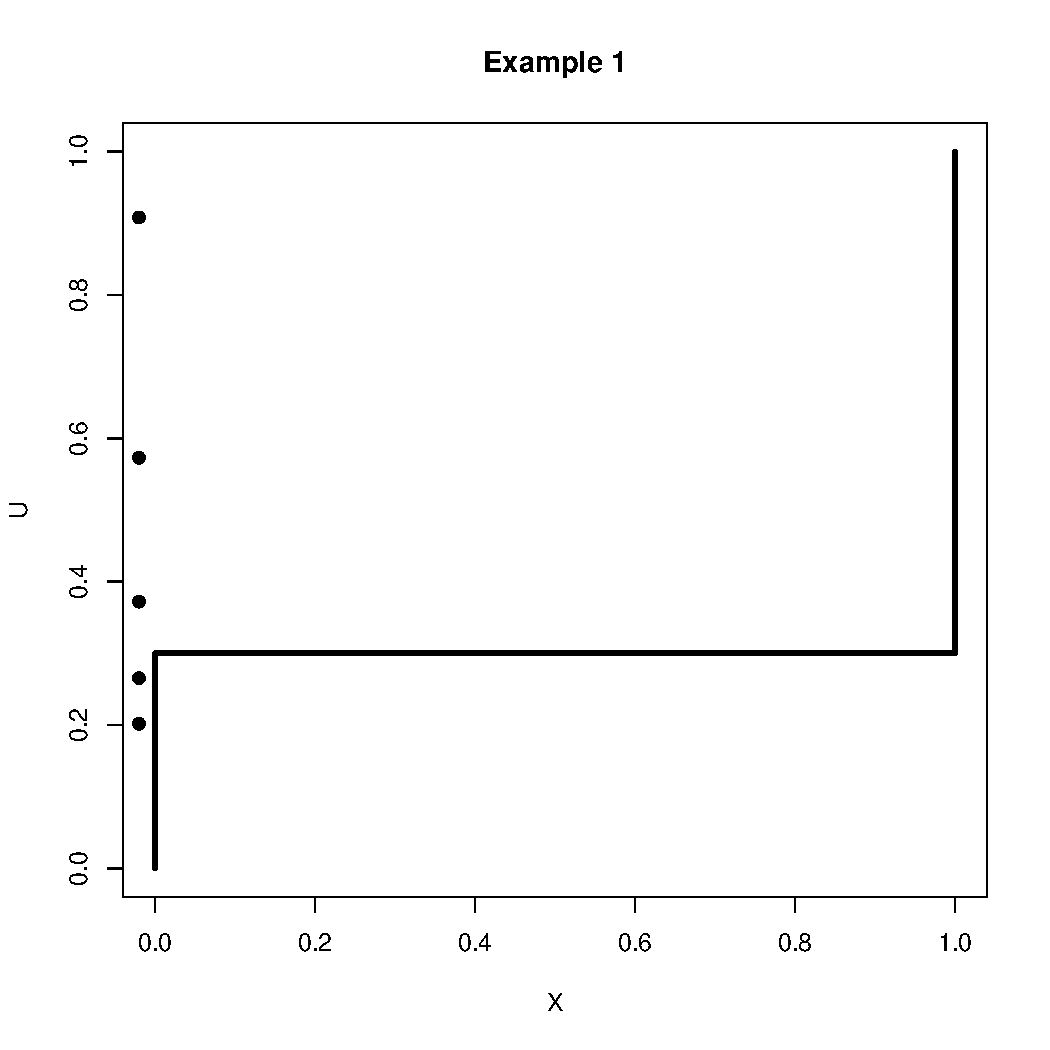
\includegraphics[height=7cm]{./Pics/d1p1.pdf}
                \end{center}
              \end{frame}

              \begin{frame}
                \frametitle{Direct Methods}
                \framesubtitle{Visualization: Example 1}
                \begin{center}
                  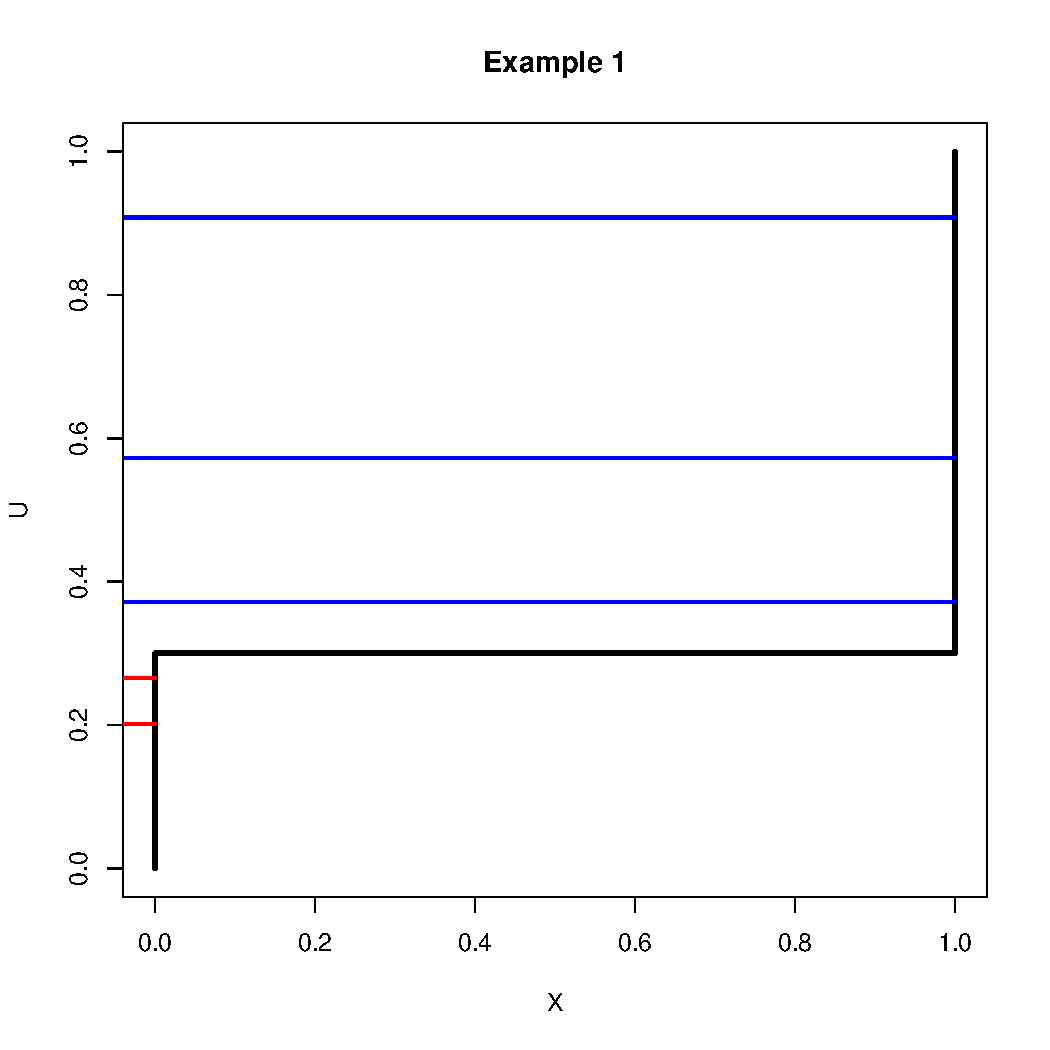
\includegraphics[height=7cm]{./Pics/d1p2.pdf}
                \end{center}
              \end{frame}

              \begin{frame}
                \frametitle{Direct Methods}
                \framesubtitle{Visualization: Example 1}
                \begin{center}
                  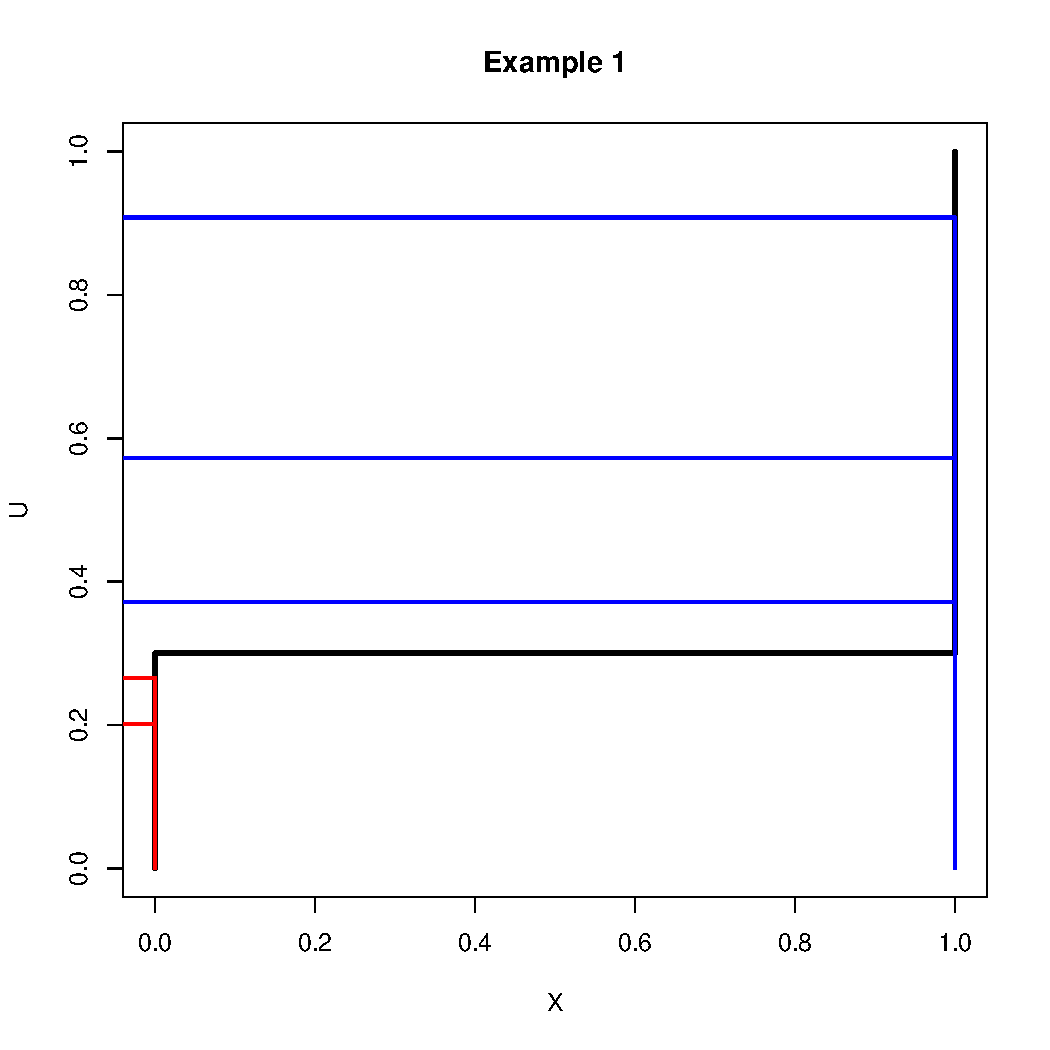
\includegraphics[height=7cm]{./Pics/d1p3.pdf}
                \end{center}
              \end{frame}

              \begin{frame}
                \frametitle{Direct Methods}
                \framesubtitle{Visualization: Example 2}
                \begin{center}
                  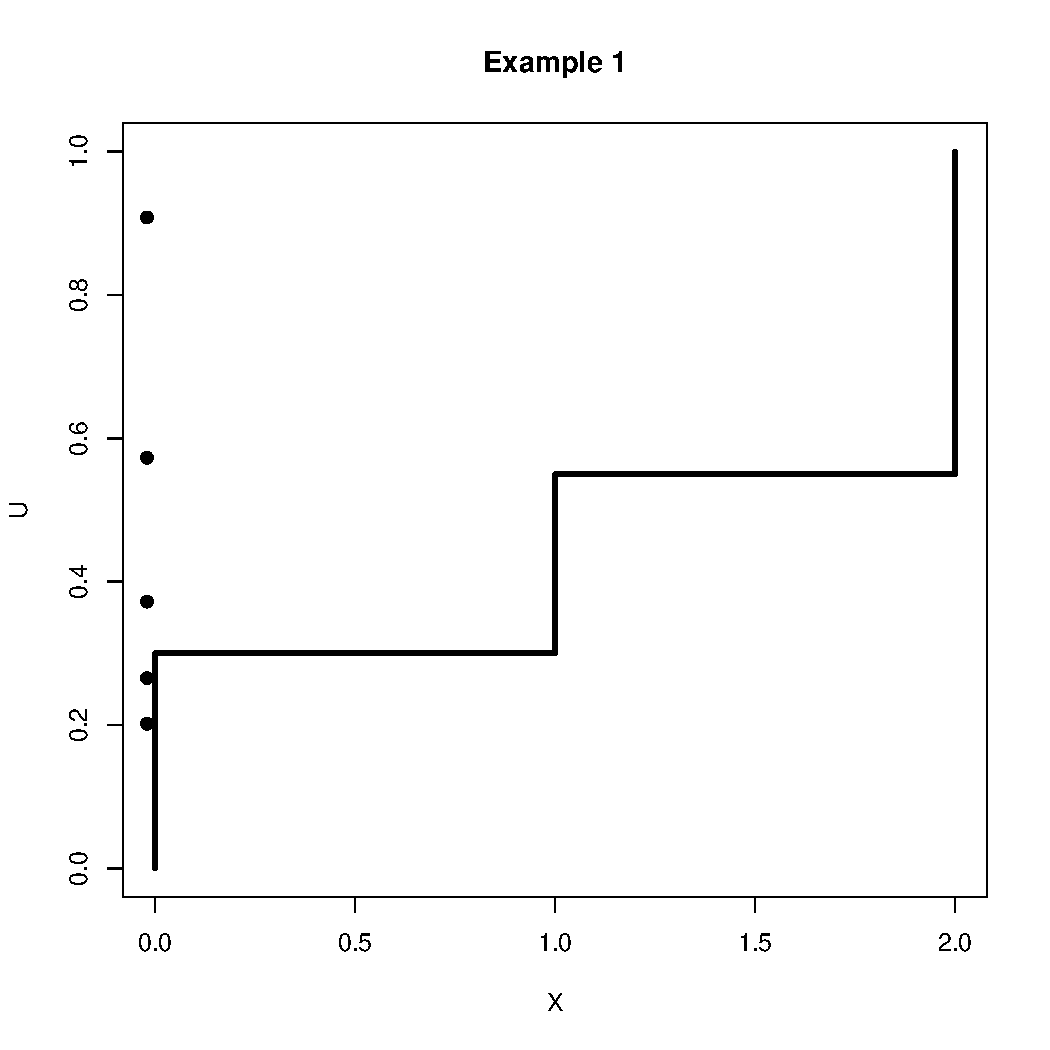
\includegraphics[height=7cm]{./Pics/d2p1.pdf}
                \end{center}
              \end{frame}

              \begin{frame}
                \frametitle{Direct Methods}
                \framesubtitle{Visualization: Example 2}
                \begin{center}
                  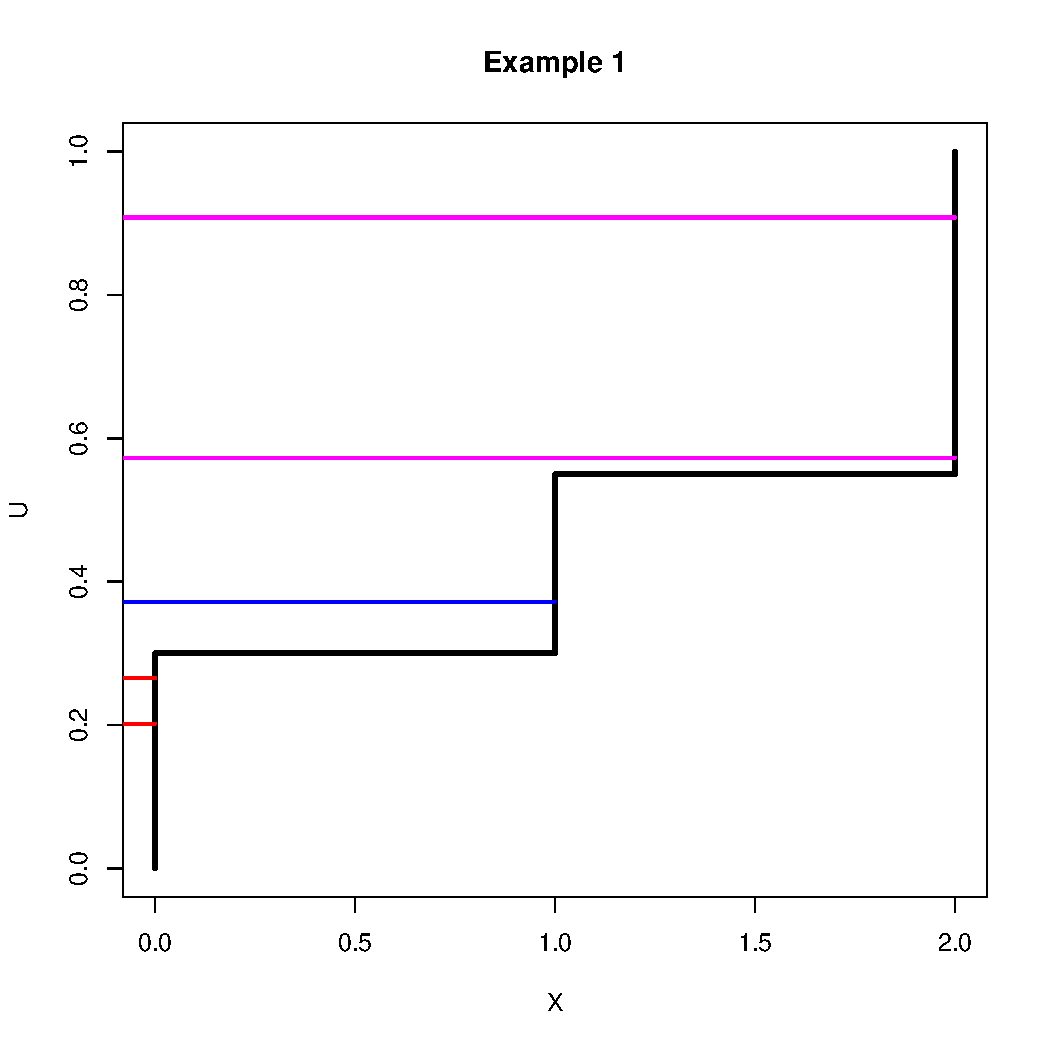
\includegraphics[height=7cm]{./Pics/d2p2.pdf}
                \end{center}
              \end{frame}

              \begin{frame}
                \frametitle{Direct Methods}
                \framesubtitle{Visualization: Example 2}
                \begin{center}
                  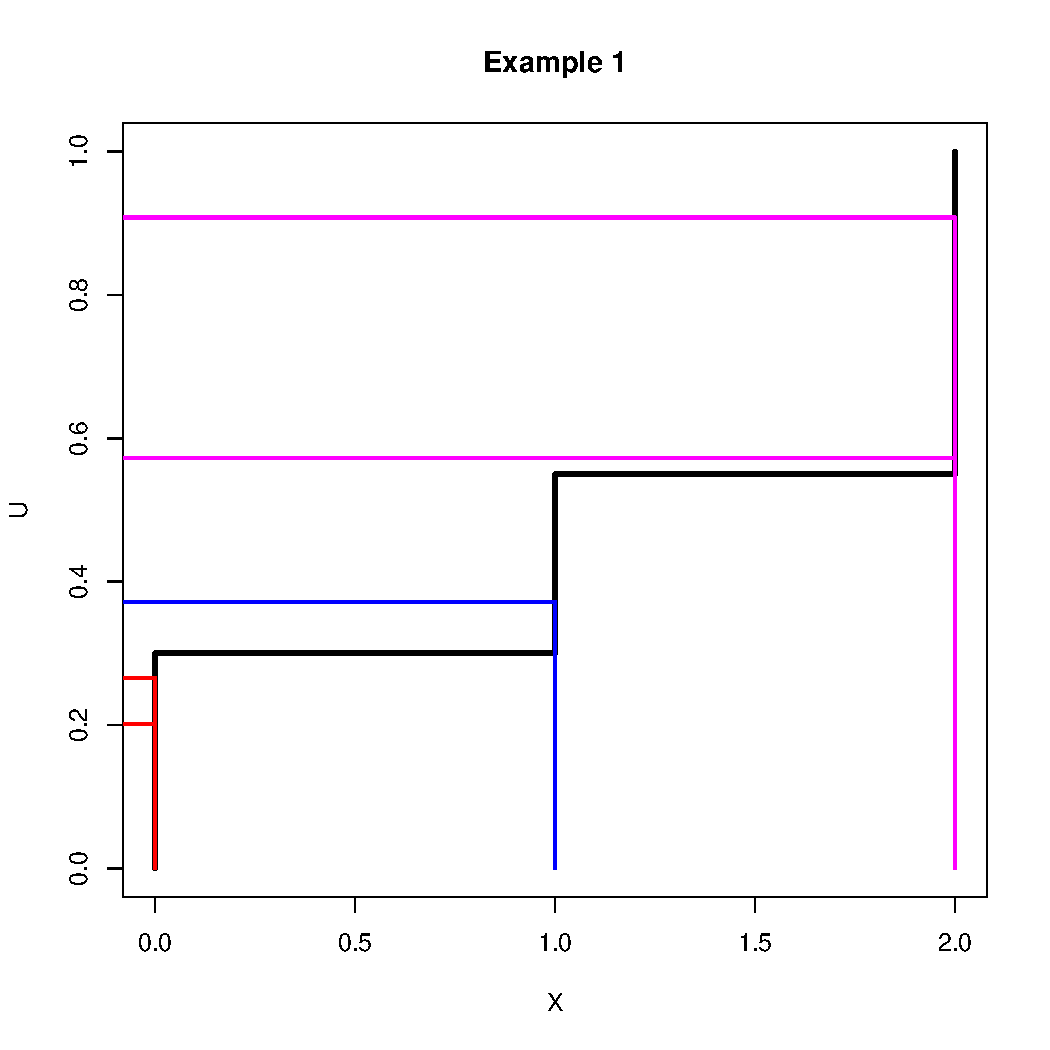
\includegraphics[height=7cm]{./Pics/d2p3.pdf}
                \end{center}
              \end{frame}


              \begin{frame}
                \frametitle{Direct Methods}
                \framesubtitle{Continuous Case}
                \begin{itemize}
                \item How do we extend this idea to the continuous case?

                \item What was the step function in our discrete example?

                \item It is the {\bf cumulative distribution function (cdf)}

                \item Can we replace the discrete cdf with a continuous cdf?

                \item Yes!
                \end{itemize}
              \end{frame}

              \begin{frame}
                \frametitle{Direct Methods}
                \framesubtitle{Visualization: Continuous}
                \begin{center}
                  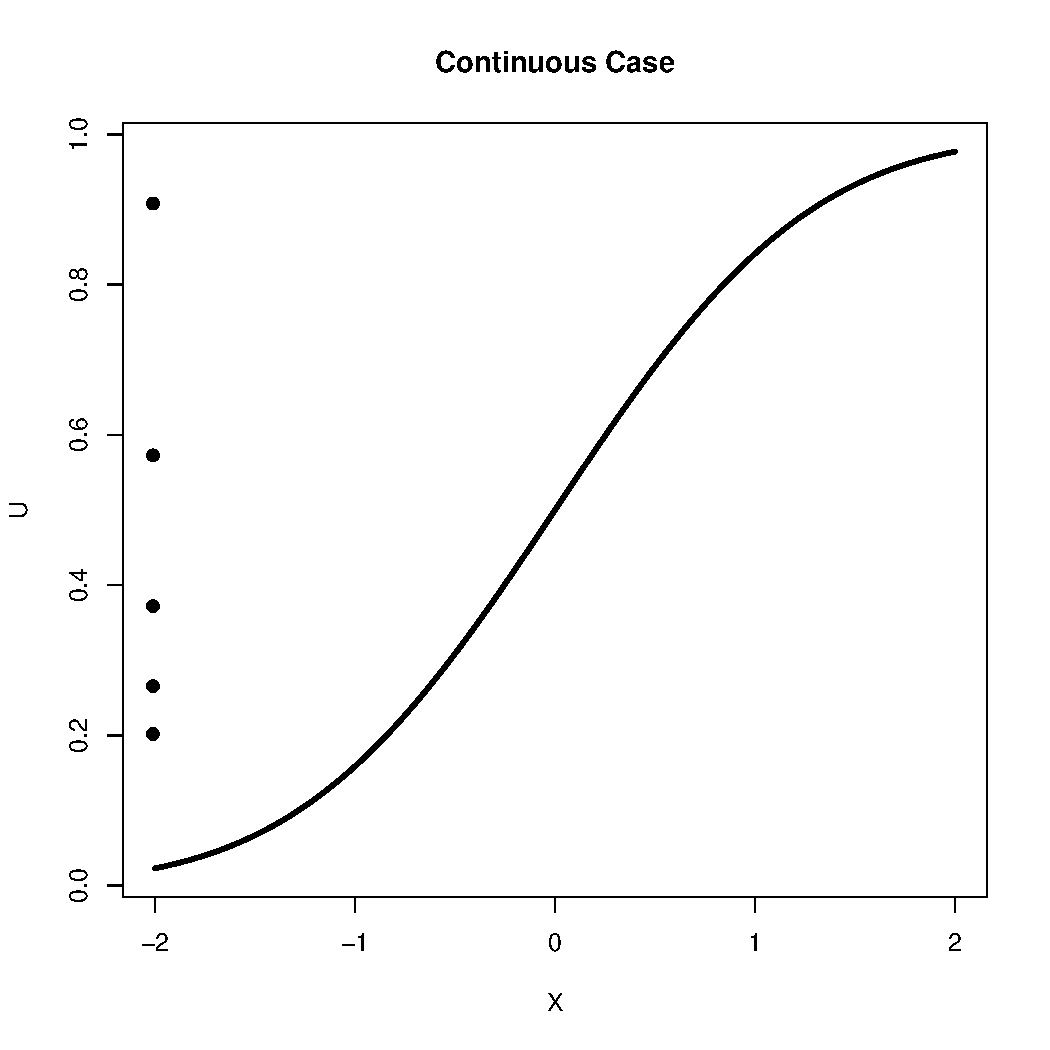
\includegraphics[height=7cm]{./Pics/cp1.pdf}
                \end{center}
              \end{frame}

              \begin{frame}
                \frametitle{Direct Methods}
                \framesubtitle{Visualization: Continuous}
                \begin{center}
                  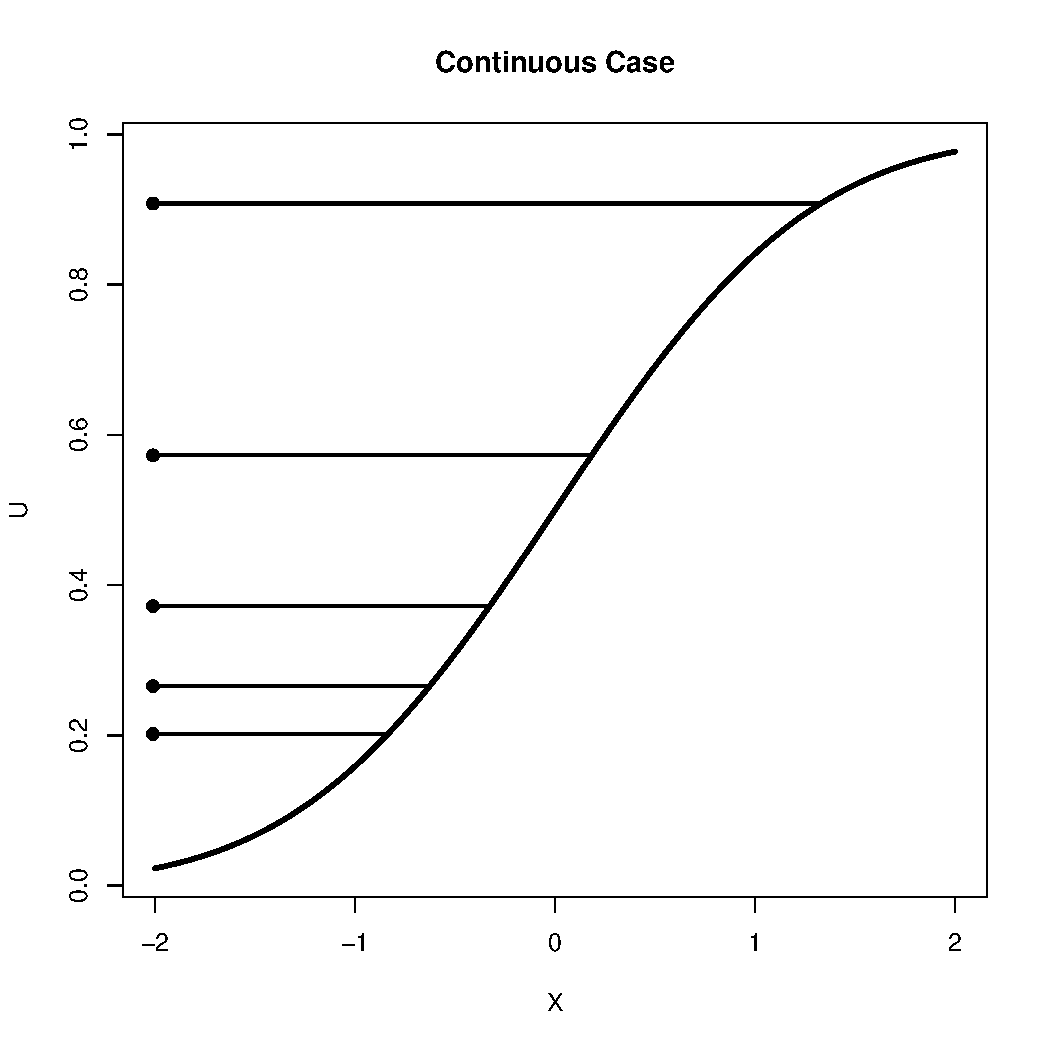
\includegraphics[height=7cm]{./Pics/cp2.pdf}
                \end{center}
              \end{frame}

              \begin{frame}
                \frametitle{Direct Methods}
                \framesubtitle{Visualization: Continuous}
                \begin{center}
                  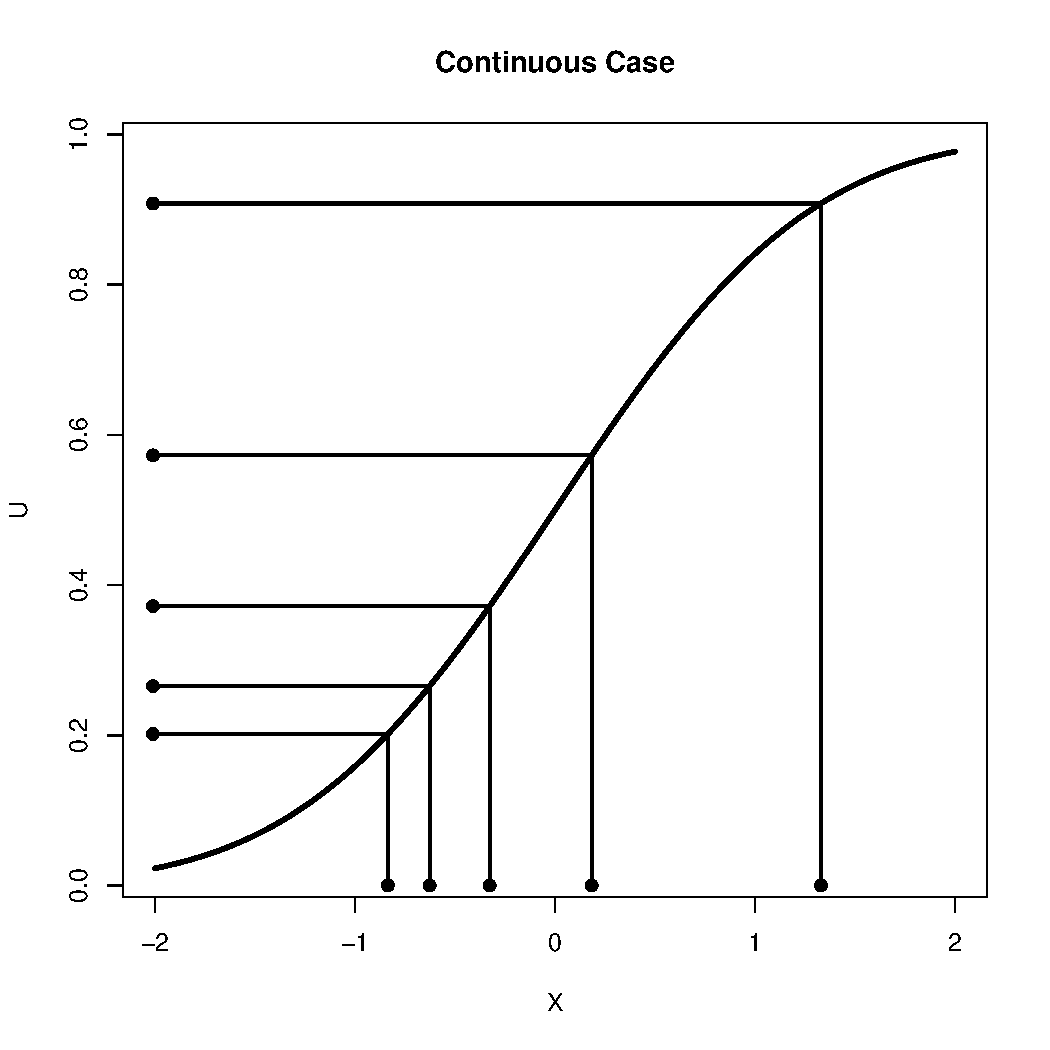
\includegraphics[height=7cm]{./Pics/cp3.pdf}
                \end{center}
              \end{frame}

              \begin{frame}
                \frametitle{Direct Methods}
                \framesubtitle{Continuous Case}
                \begin{itemize}
                \item The cdf, $F(X)$ takes values of $X$ and gives a value between $0$ and $1$

                \item Here we take values between $0$ and $1$ and get a value of $X$

                \item What function do we use?

                \item We use the {\bf Inverse cdf}
                \end{itemize}
              \end{frame}



              \begin{frame}
                \frametitle{Direct Methods}
                \framesubtitle{Probability Integral Transform}

                \begin{itemize}
                \item If $Y$ is a continuous random variable with cdf $F(y)$ , then
                  the random variable $F_y^{-1}(U)$, where $U \sim uniform(O, 1)$, has
                  distribution $F(y)$.

                \item \textbf{Example:} If $Y \sim exponential(A)$, then the probability density
                  function (PDF) is
                  \begin{equation*}
                    f(x;\lambda) = \begin{cases} \lambda e^{-\lambda x} & x \ge 0, \\ 0 & x < 0. \end{cases}
                  \end{equation*}
                  and the cumulative distribution function (CDF) is given by
                  \begin{equation*}
                    F(x;\lambda) = \begin{cases} 1-e^{-\lambda x} & x \ge 0, \\ 0 & x < 0. \end{cases}
                  \end{equation*}
                  Then
                  \begin{equation*}
                    F_Y^{-1}(U) = -\log(1-U)/\lambda
                  \end{equation*}
                  is an exponential random variable.

                \item Thus, if we generate $U_1,..., U_n$ as iid uniform random
                  variables, $-\lambda (1-U_i)$, are iid exponential random
                  variables with parameter $\lambda$.

                \end{itemize}

              \end{frame}

              \section{Indirect Methods}


              \begin{frame}{Indirect simulation}
                \begin{itemize}
                \item What if the cumulative distribution function is difficult to invert, or not even available?

                \item How to invert the cdf of a standard normal distribution?

                  \begin{equation}
                    F(x)=\int_{-\infty}^{x}(2\pi)^{-1/2}e^{-x^2/2}dx
                  \end{equation}

                \item It is still possible to simulate from this distribution?

                \item If the {\bf density} is available, then the answer is YES!
                \end{itemize}
              \end{frame}



              \begin{frame}{The student's \emph{t} distribution}
                \begin{itemize}
                \item The student's \emph{t} distribution has density function
                  \begin{equation*}
                    f(t) = \frac{\Gamma(\frac{\nu+1}{2})} {\sqrt{\nu\pi}\,\Gamma(\frac{\nu}{2})} \left(1+\frac{t^2}{\nu} \right)^{\!-\frac{\nu+1}{2}}
                  \end{equation*}

                \item It is similar to the normal but has fatter tails.

                \item It is not so easy to simulate from this distribution using the
                  direct method.
                \end{itemize}
              \end{frame}

              \begin{frame}{Normal (red) vs Student's t (blue)}
                \begin{center}
                  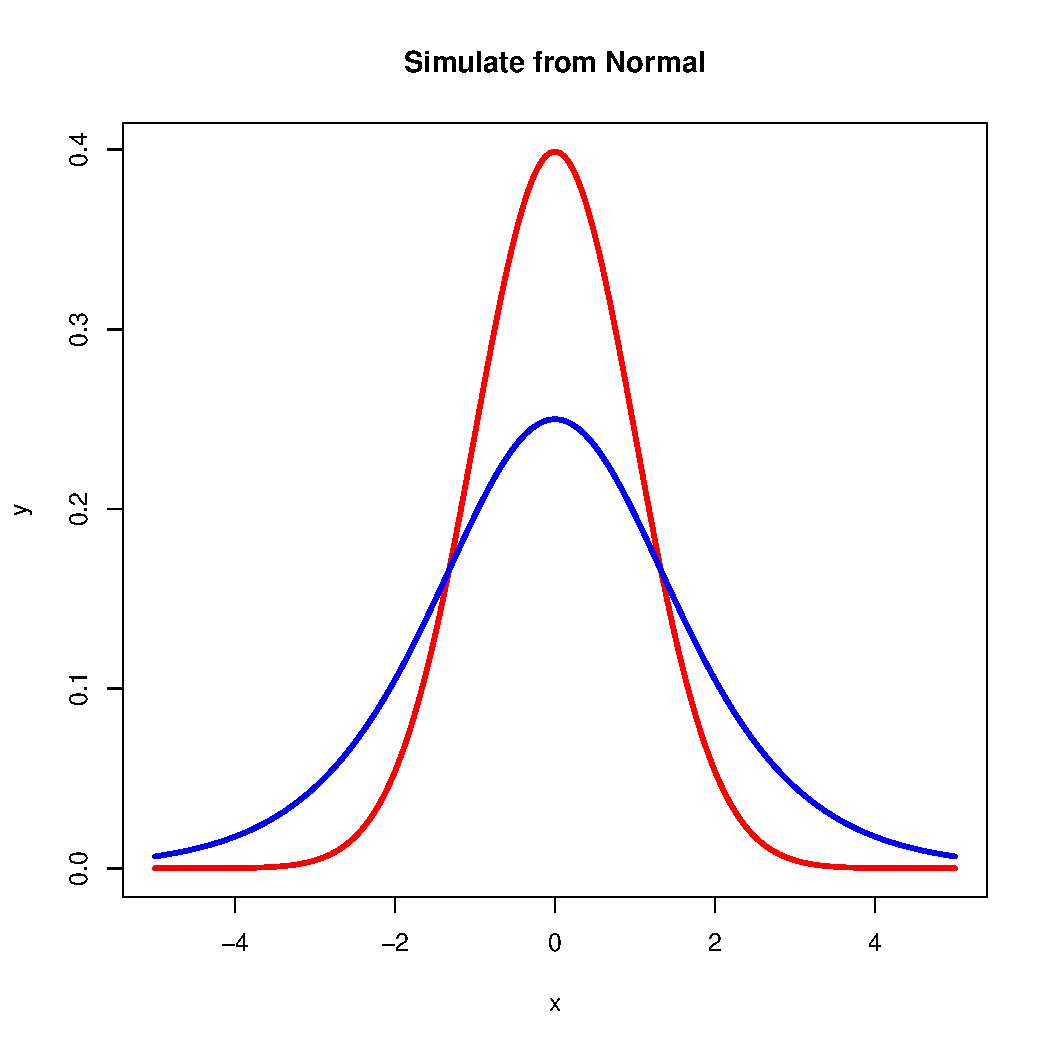
\includegraphics[height=7cm]{./Pics/nmlg1.pdf}
                \end{center}
              \end{frame}

              \begin{frame}{Normal vs Student's t}
                \begin{center}
                  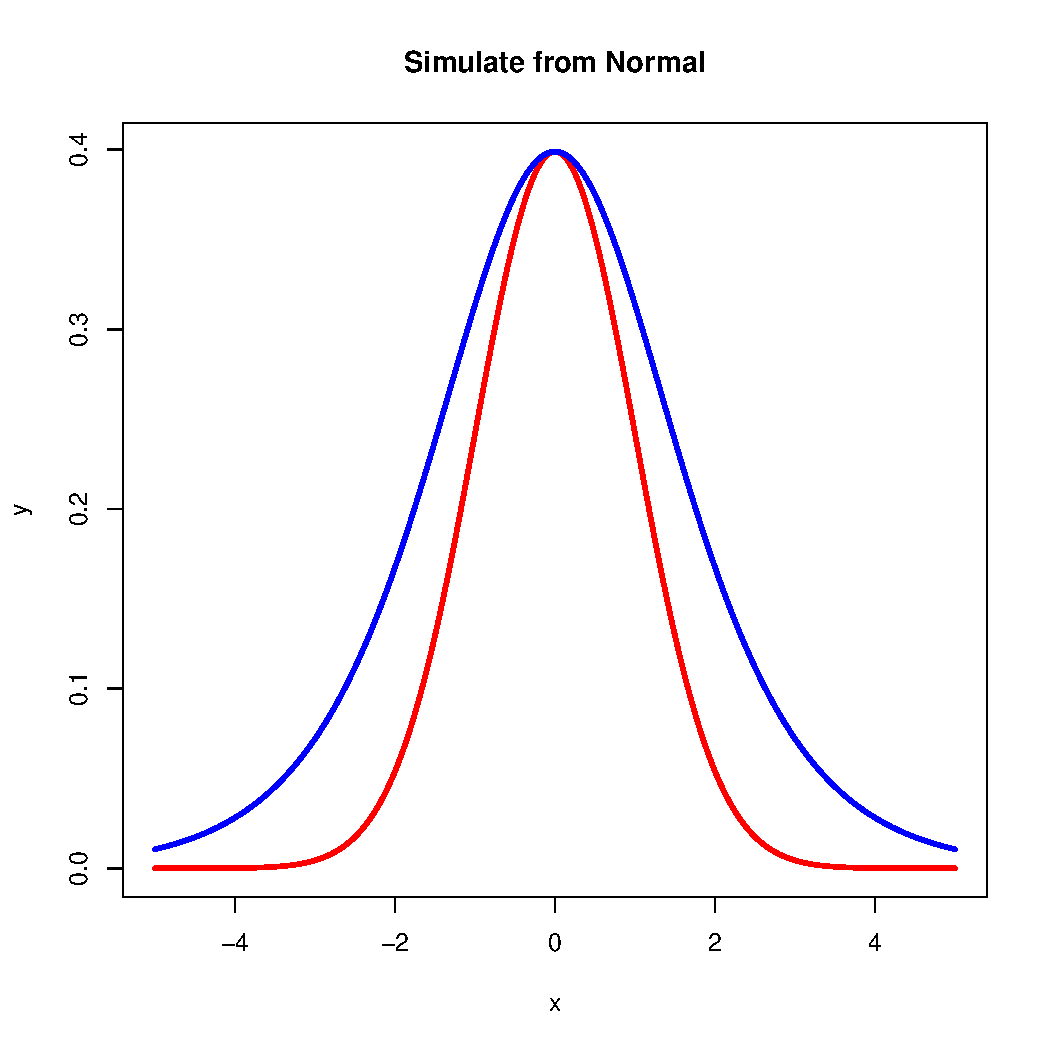
\includegraphics[height=7cm]{./Pics/nmlg2.pdf}
                \end{center}
              \end{frame}

              \begin{frame}{Normal vs Student's t}
                \begin{center}
                  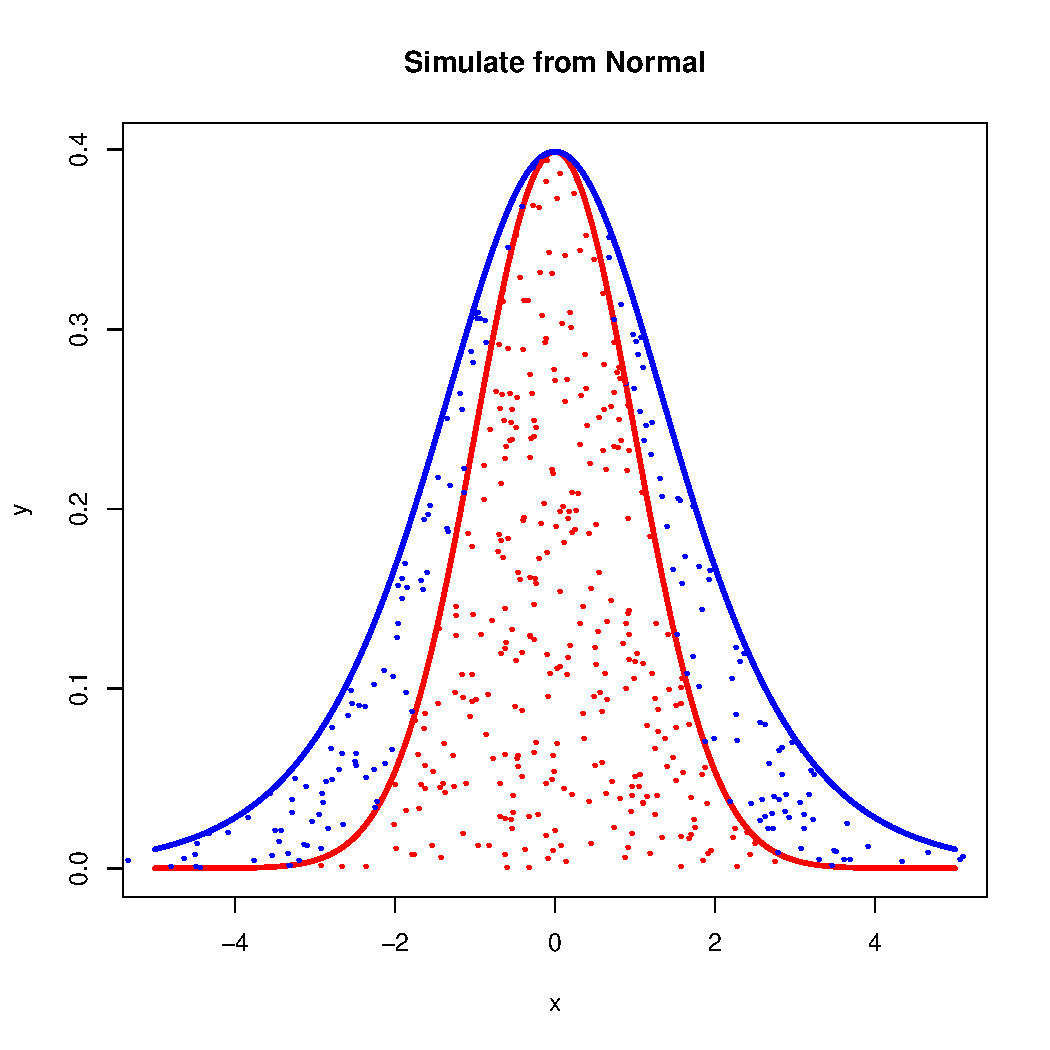
\includegraphics[height=7cm]{./Pics/nmlg3.pdf}
                \end{center}
              \end{frame}


              \begin{frame}{The idea}
                \begin{itemize}
                \item Let $f_y(x)$ be the {\bf target distribution} and $f_v(v)$ be the {\bf proposal distribution}

                \item Simulate an $x$-coordinate from the proposal $f_v(x)$

                \item Simulate a y-coordinate from $U(0, M*f_v(x))$

                \item Reject any points that are not `inside' $f_y(x)$
                \end{itemize}
              \end{frame}



              \begin{frame}
                \frametitle{Indirect Methods}
                \framesubtitle{Reject and accept method}

                \begin{itemize}
                \item \textbf{Theorem:} Let $Y \sim f_Y(y)$ and $V \sim f_v(v)$,
                  where $f_Y$ and $f_V$ have common support with
                  \begin{equation*}
                    M = sup_y f_Y(y)/f_V(y) < \infty.
                  \end{equation*}
                  To generate a random variable $Y\sim f_Y$, we do the following
                  steps
                  \begin{enumerate}
                  \item Generate $U\sim uniform(0,1)$ and $V\sim f_V$ independently.
                  \item If
                    \begin{equation*}
                      U < \frac{1}{M} \frac{f_Y(V)}{f_V(V)}
                    \end{equation*}
                    set $Y = V$; otherwise, return to step 1.
                  \end{enumerate}

                \end{itemize}
              \end{frame}


              \begin{frame}
                \frametitle{Indirect Methods}
                \framesubtitle{Reject and accept method}
                \begin{center}
                  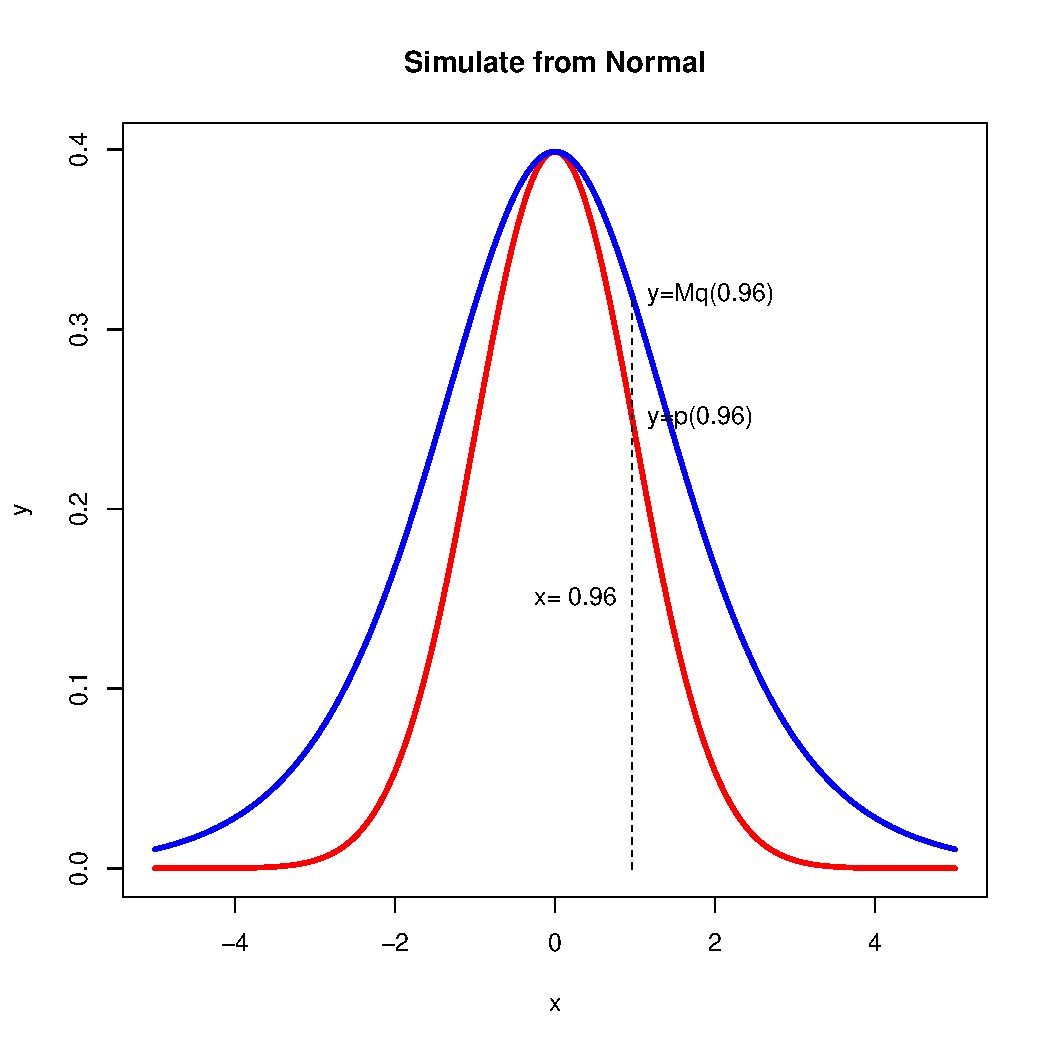
\includegraphics[height=7cm]{./Pics/nmlg4.pdf}
                \end{center}
              \end{frame}
              \begin{frame}
                \frametitle{Indirect Methods}
                \framesubtitle{Reject and accept method}
                \begin{center}
                  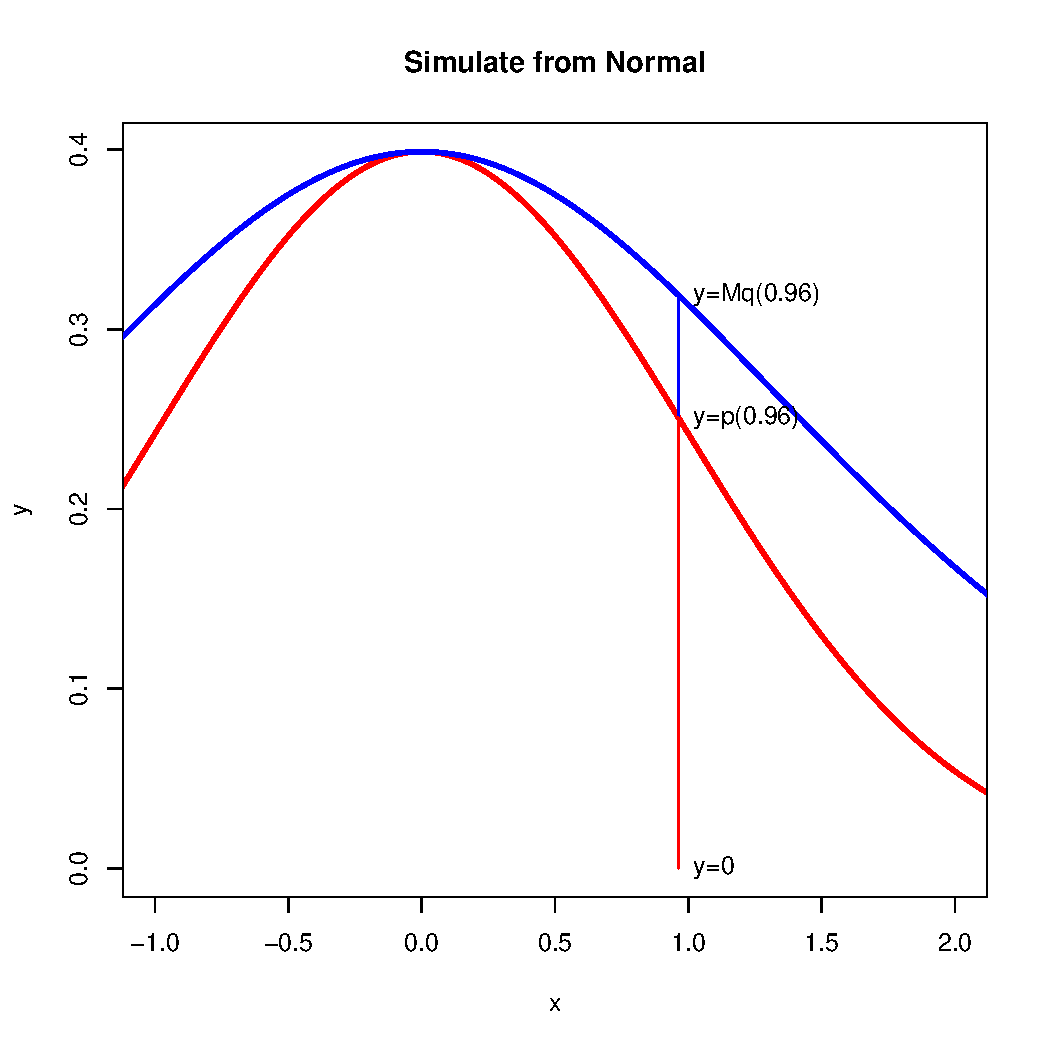
\includegraphics[height=7cm]{./Pics/nmlg5.pdf}
                \end{center}
              \end{frame}
              \begin{frame}
                \frametitle{Indirect Methods}
                \framesubtitle{Reject and accept method}
                \begin{center}
                  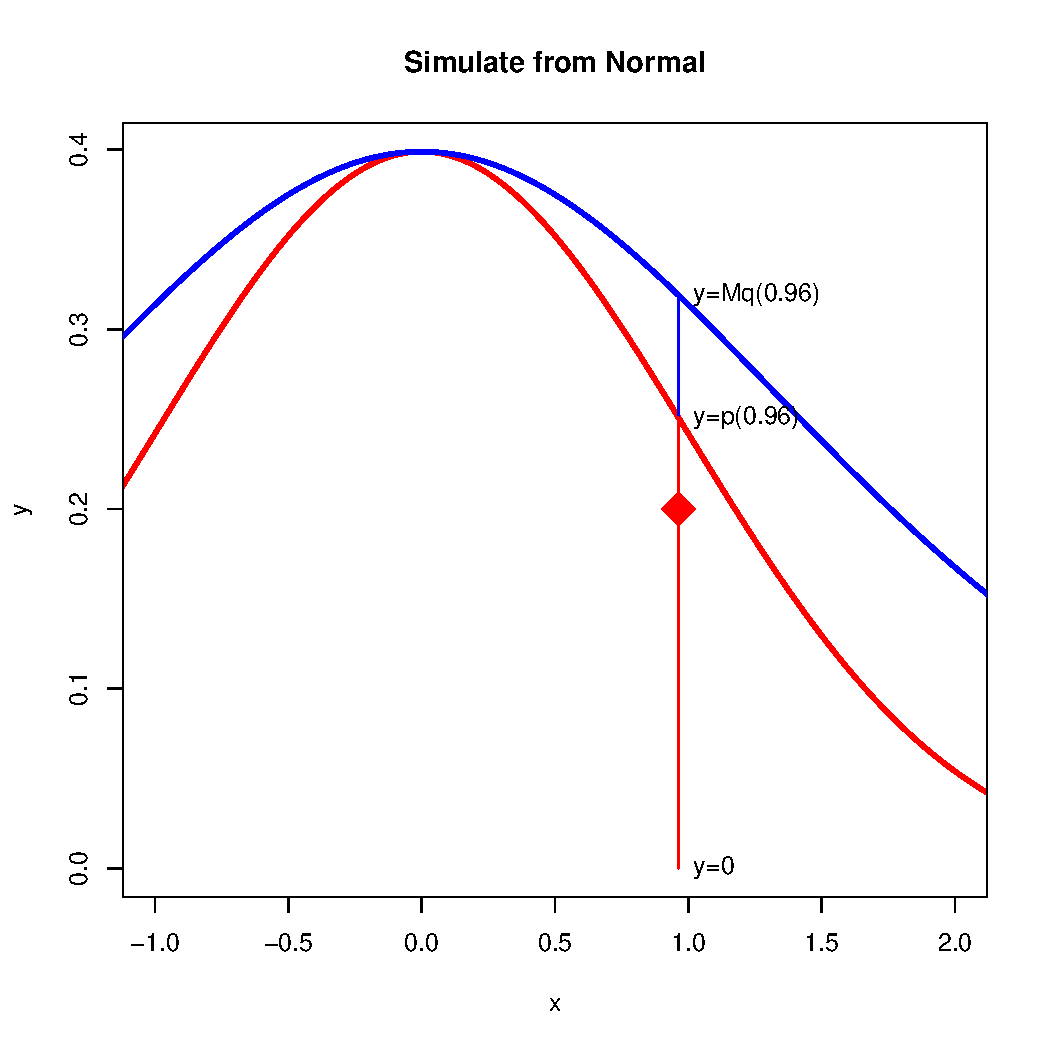
\includegraphics[height=7cm]{./Pics/nmlg6.pdf}
                \end{center}
              \end{frame}
              \begin{frame}
                \frametitle{Indirect Methods}
                \framesubtitle{Reject and accept method}
                \begin{center}
                  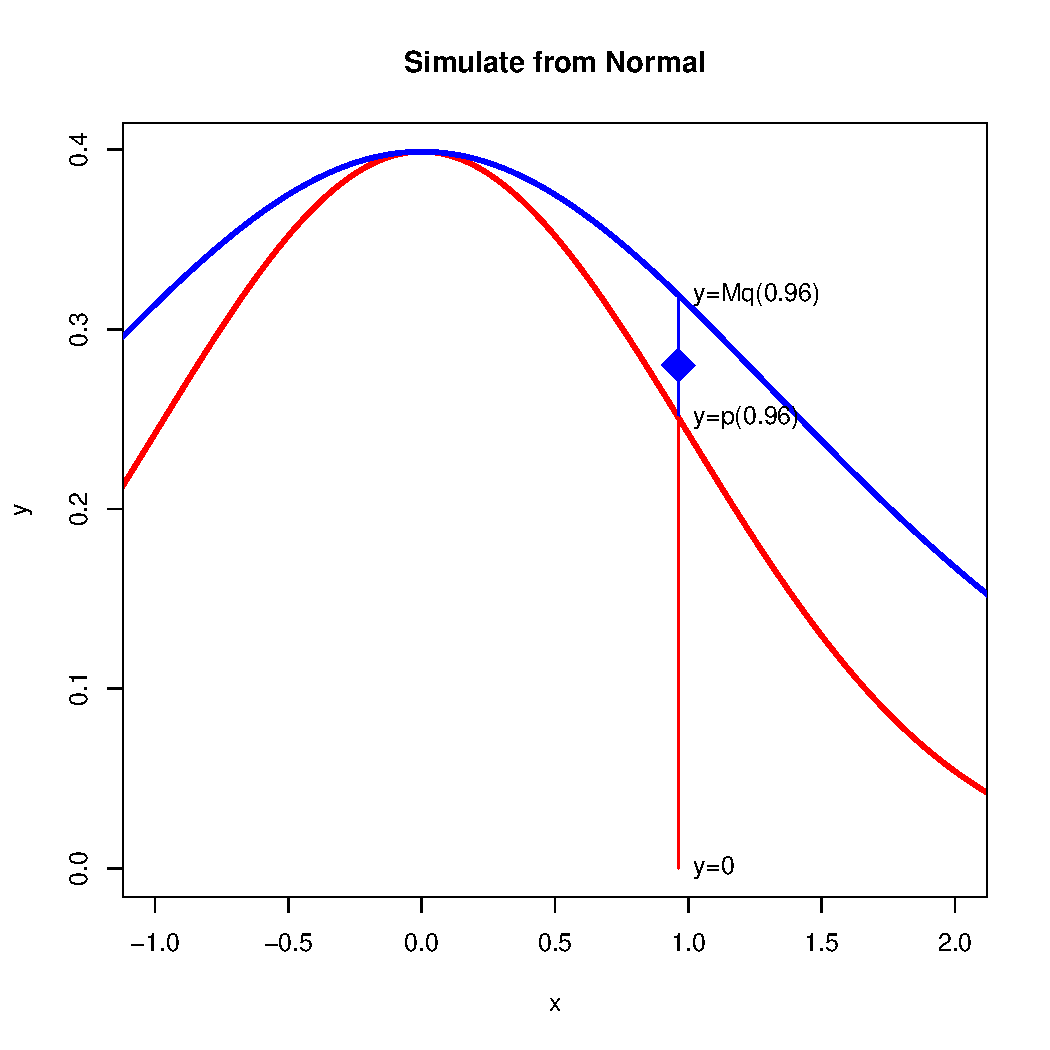
\includegraphics[height=7cm]{./Pics/nmlg7.pdf}
                \end{center}
              \end{frame}


              \begin{frame}
                \frametitle{Indirect Methods}
                \framesubtitle{Reject and accept method: the proof}
                \vspace{-0.6cm}
                \begin{align*}
                  P(V\leq y |stopping~rule)&= P(V\leq y | U < \frac{1}{M} \frac{f_Y(V)}{f_V(V)})\\
                                           &= \frac{P(V\leq y , U < \frac{1}{M} \frac{f_Y(V)}{f_V(V)})}{P(U <
                                             \frac{1}{M} \frac{f_Y(V)}{f_V(V)})}\\
                                           &= \frac{\int_{-\infty}^y\int_0^{\frac{1}{M}
                                             \frac{f_Y(V)}{f_V(V)}}du~f_V(v)dv}{\int_{-\infty}^{\infty}\int_0^{\frac{1}{M}
                                             \frac{f_Y(V)}{f_V(V)}}du~f_V(v)dv}\\
                                           &= \frac{\int_{-\infty}^y\frac{1}{M}
                                             \frac{f_Y(V)}{f_V(V)}f_V(V)dv}{\int_{-\infty}^{\infty}\frac{1}{M}
                                             \frac{f_Y(V)}{f_V(V)}f_V(V)dv}\\
                                           &=\int_{-\infty}^y f_Y(v)dv
                \end{align*}

                \begin{itemize}
                \item Can have any $M$? In fact $M$ shows the efficiency of the sampling
                  algorithm, i.e.  $M= 1/P(stopping~rule)$.
                \end{itemize}
              \end{frame}



              \begin{frame}
                \frametitle{Indirect Methods}
                \framesubtitle{Choosing $f_v(x)$ and $M$}
                \begin{itemize}
                \item Two things are necessary for the accept/reject algorithm to work:
                  \begin{enumerate}
                  \item The domain of $p(x)$ and the domain of $q(x)$ MUST be the same.
                  \item The value of $M$ must satisfy $M\geq \sup_x p(x)/q(x)$
                  \end{enumerate}
                \item The algorithm will be more {\bf efficient} if:
                  \begin{enumerate}
                  \item The proposal $q(x)$ is a good approximation to $p(x)$
                  \item The value of $M$ is $M=\sup_x p(x)/q(x)$
                  \end{enumerate}
                \end{itemize}
              \end{frame}

              \begin{frame}
                \frametitle{Indirect Methods}
                \framesubtitle{A look at $f_y(x)/f_v(x)$}
                \begin{center}
                  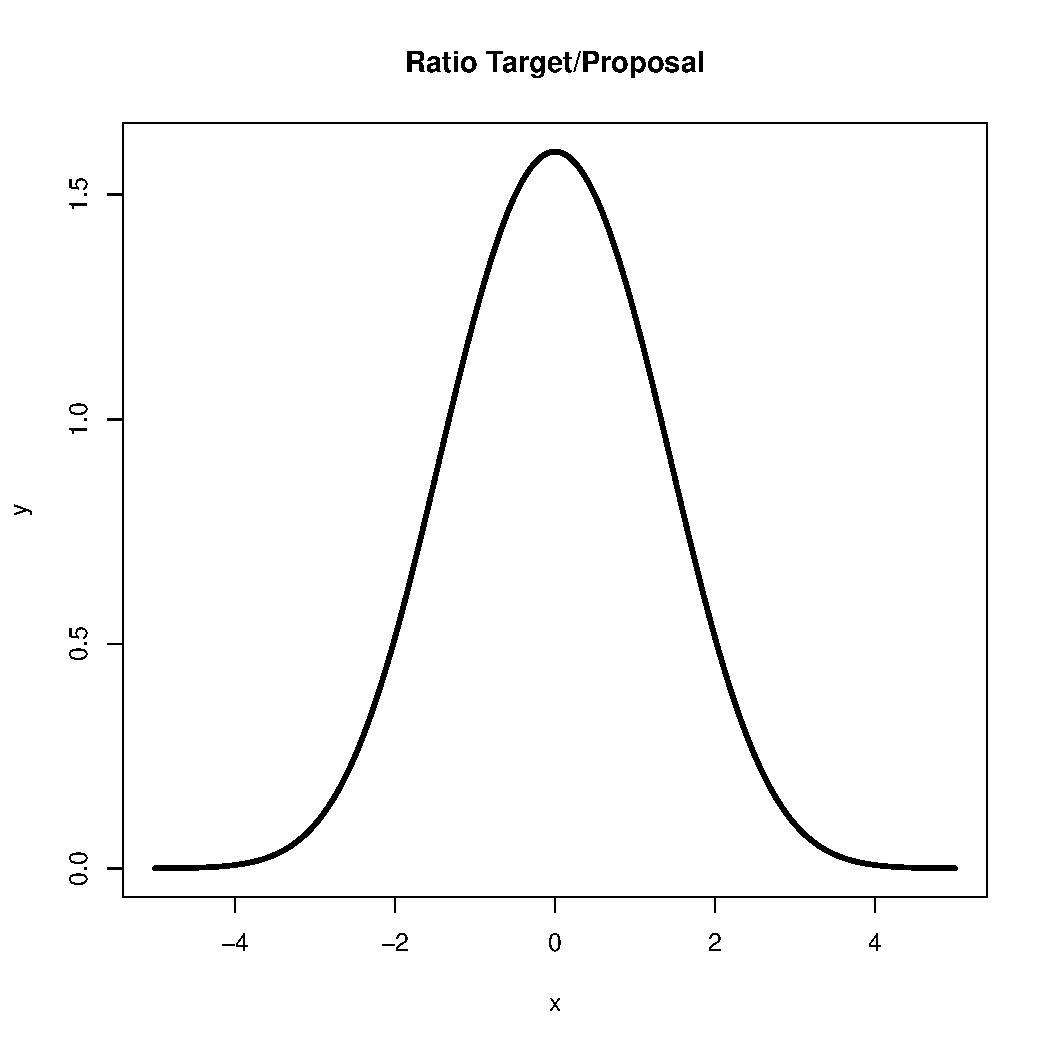
\includegraphics[height=7cm]{./Pics/rat1.pdf}
                \end{center}
              \end{frame}


              \begin{frame}
                \frametitle{Indirect Methods}
                \framesubtitle{A look at $f_y(x)/f_v(x)$}

                \begin{center}
                  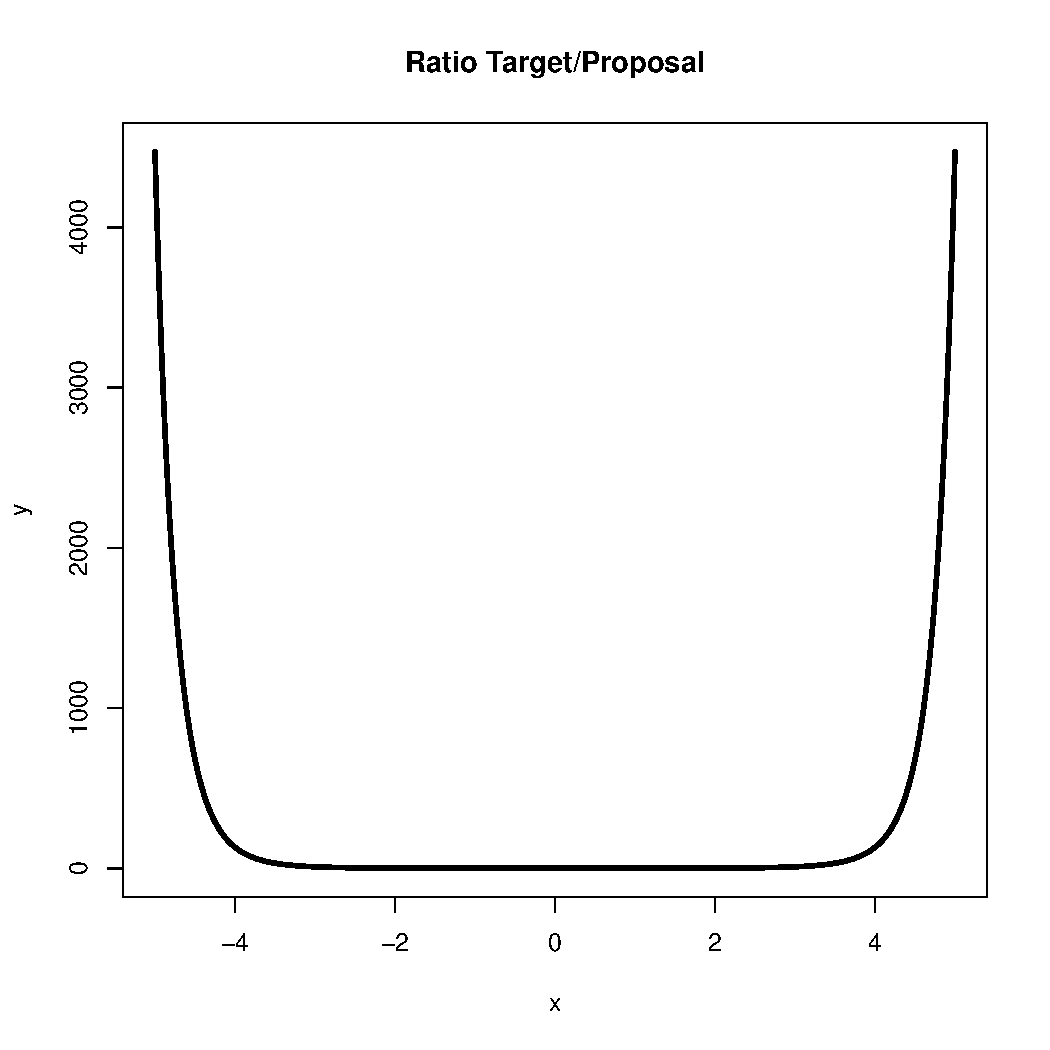
\includegraphics[height=7cm]{./Pics/rat2.pdf}
                \end{center}
              \end{frame}



              \begin{frame}{Normalizing Constant and Kernel}
                \begin{itemize}
                \item Today we saw many density functions $f(x)$
                \item Many density functions can written as $f(x)=k\tilde{f}(x)$
                \item The part $k$ is called the {\color{blue} normalizing constant} and
                  the part $\tilde{f}(x)$ is called the {\color{red}
                    kernel}.
                \item For example the standard normal distribution is
                  \alt<2>
                  {\begin{equation}
                      p(x)={\color{blue}(2\pi)^{-1/2}}{\color{red}e^{-x^2/2}}
                    \end{equation}}
                  {\begin{equation}
                      p(x)=(2\pi)^{-1/2}e^{-x^2/2}
                    \end{equation}}

                \end{itemize}
              \end{frame}
              \begin{frame}{Normalizing Constant and Kernel}
                What are the {\color{blue} normalizing constant}
                and
                {\color{red} kernel}
                of the Beta function?

                \begin{equation}
                  \mbox{Beta}(x;a,b)={\color{blue}\frac{\Gamma(a+b)}{(\Gamma(a)\Gamma(b))}}{\color{red}x^{a-1}(1-x)^{b-1}}
                \end{equation}

              \end{frame}
              \begin{frame}{Accept/Reject and the normalising constant}
                \begin{itemize}
                \item An advantage of the Accept/Reject algorithm is that is works, even if the normalizing constant is unavailable.

                \item Only the kernel is needed.

                \item There are many examples where the normalising constant is either unavailable or difficult to compute.

                \item This often happens in Bayesian analysis
                \end{itemize}
              \end{frame}



              \begin{frame}
                \frametitle{Suggested Reading}

                \begin{itemize}
                \item Jones (2009), \textbf{Chapter 18}


                  % \emph{Monte Carlo Statistical Methods} Book by Christian P Robert and George
                  % Casella. (2004 edition)

                \end{itemize}

              \end{frame}


            \end{document}
